\documentclass[../defence.tex]{subfiles}
\begin{document}

  \begin{frame}{Annormaler ganzzahliger Quanten Hall Effekt (QHE) in Graphen II}
    \onslide<1->{
    \begin{columns}[onlytextwidth, T]
      \column{\dimexpr\linewidth / 2}
        \begin{block}{Laughlins Gedankenexperiment für lokalisierte Zustände}
          \onslide<2->{
            \begin{equation*}
              I=c\frac{\delta E}{\delta \Phi},
            \end{equation*}
            $E$-Gesamtenergie des Systems,\\
            $\Phi$-Magnetischer Fluss\\
            \onslide<3>{
            $\rightarrow$ betrachte Flussänderung $\delta \Phi = hc/e$ (eine Flussquante)
            }
          }
        \end{block}
      \column{\dimexpr\linewidth / 2}
        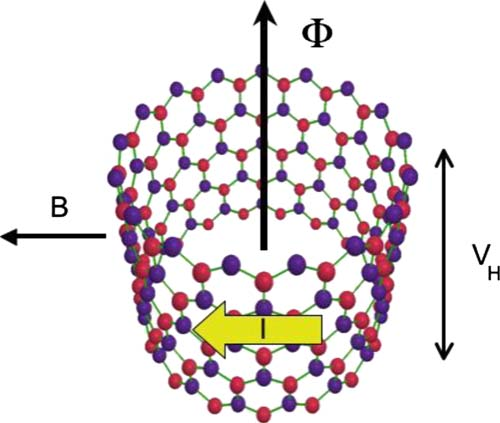
\includegraphics[width=\linewidth]{images/laughlin.png}
        \cite{castro2009}
    \end{columns}}
    \note{
      \begin{itemize}
        \item Lorentzkraft erzeugt Hall-Spannung orthogonal zu Feld und Strom
        \item Lokalisierte Zustände reagieren \textbf{nicht} auf Änderungen des Flusses $\Phi$ (nur die delokalisierten)
        \item Alle Zustände unter dem chemischen Potential vor und nach Änderung von $\Phi$ besetzt
        \item \textbf{Aber:} Eine ganzzahlige Anzahl Zustände kommt auf einer Seite rein und verlässt den Zylinder auf der anderen Seite
      \end{itemize}
    }
  \end{frame}

\end{document}
